\documentclass{beamer}
\usepackage[utf8]{inputenc}

\usetheme{Madrid}
\usecolortheme{default}
\useinnertheme{circles}

\definecolor{Logo1}{rgb}{0.208, 0.2865, 0.373}
\definecolor{Logo2}{rgb}{0.000, 0.674, 0.863}

\setbeamercolor*{palette primary}{bg=Logo1, fg=white}
\setbeamercolor*{palette secondary}{bg=Logo2, fg=white}
\setbeamercolor*{palette tertiary}{bg=white, fg=Logo1}
\setbeamercolor*{palette quaternary}{bg=Logo1,fg=white}
\setbeamercolor{structure}{fg=Logo1} % itemize, enumerate, etc
\setbeamercolor{section in toc}{fg=Logo1} % TOC sections

%-----------------------------------------------------------
\title[]{Cloud Computing Case Study: Amazon Web Services}
\author[]{Debanjan Kola, Sauvik Dutta, Sankha Ghosh, Somnath Ganguly}

\institute[]{
  Department of Computer Science\\
  Ramakrishna Mission Vivekananda Centenary College
}
\date[]{September 2024}


%\logo{
\includegraphics[height=.5cm]{logo-footer.png}}


\AtBeginSection[]
{
  \begin{frame}
    \frametitle{Table of Contents}
    \tableofcontents[currentsection]
  \end{frame}
}
%------------------------------------------------------------


\begin{document}


\frame{\titlepage}


\begin{frame}
\frametitle{Table of Contents}
\tableofcontents
\end{frame}



\section{AWS as Platform as a Service (PaaS)}

\begin{frame}
\frametitle{What is PaaS?}
\begin{block}{Defintion}
	Platform as a Service (PaaS) is a cloud computing model that provides a platform allowing customers to develop, run, and manage applications without the complexity of building and maintaining the underlying infrastructure.
\end{block}
\end{frame}


\begin{frame}
	\frametitle{PaaS of AWS}
	\begin{examples}{AWS Services that belongs to PaaS}
		\begin{itemize}
			\item AWS Lambda
			\item Amazon Polly
		\end{itemize}
	\end{examples}		
\end{frame}

\begin{frame}
	\frametitle{AWS Lambda}
	\begin{block}{Defintion}
		AWS Lambda is a serverless computing service that lets the developers run their code in the standard runtime environment of Lambda without having to worry about server handling with zero supervision.
	\end{block}
	
	\begin{center}
	
	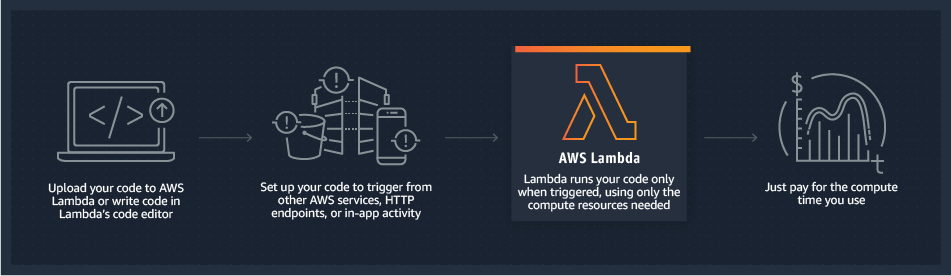
\includegraphics[scale=0.35]{product-page-diagram_Lambda-HowItWorks.68a0bcacfcf46fccf04b97f16b686ea44494303f.png}
	\end{center}
\end{frame}

\begin{frame}
\frametitle{How AWS Lambda Works}
\begin{block}{Working Principle}
User uploads the code to AWS Lambda. Whenever the Lambda function is triggered, the code will run and use the computing resources then only.
\end{block}

\begin{center}
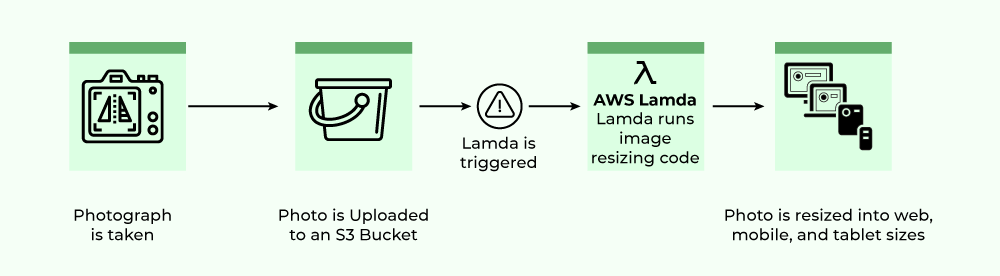
\includegraphics[scale=0.35]{aws-LAMBDA.png}
\end{center}

\end{frame}

\begin{frame}
	\frametitle{AWS Lambda Functions}
	\begin{block}{Lambda Functions}
		\begin{itemize}		
			\item AWS lambda are server-less compute functions are fully managed by the AWS where developers can run there code without worrying about servers.
			\item AWS lambda functions will allow you to run the code with out provisioning or managing servers.
		\end{itemize}
	\end{block}
	
\end{frame}

\begin{frame}
	\frametitle{Where to use AWS Lambda}
	\begin{block}{}
	\begin{itemize}
		\vspace{1ex}
		\item File Processing: AWS Lambda can be triggered by using S3 Service. Whenever files are added to S3 service Lambda functions will start processing the data. \vspace{1ex} 
		\item Web Applications: AWS Lambda can be combined with web applications which will scale up and down based on the incoming traffic. \vspace{1ex}
		\item Stream Processing: Lambda functions can be used to process real-time data streaming data. \vspace{1ex}
	\end{itemize}
	\end{block}
\end{frame}

\begin{frame}
	\frametitle{Why use AWS Lambda}
	\begin{block}{}
	\begin{itemize}
		\vspace{1ex}
		\item Serverless Execution \vspace{1ex}
		\item Pay-per-use-pricing \vspace{1ex}
		\item Supports different programming languages \vspace{1ex}
		\item Auto-Scaling and High Availability \vspace{1ex}
	\end{itemize}
	\end{block}
\end{frame}

\begin{frame}
	\frametitle{Amazon Polly}
	\begin{block}{Definition}
	Amazon Polly is a cloud service that converts text into lifelike speech by using advanced deep learning technologies.
	\end{block}
	\begin{center}
		
\includegraphics[scale=0.30]{polly-social.jpg}
	\end{center}
\end{frame}

\begin{frame}
\frametitle{How Amazon Polly Works}
	\begin{block}{Working Principle}
		User provides text input and it processes the text using NTTS or TTS technique and returns the spoken version of the text in desired voice, language or format.
	\end{block}
	\begin{center}
		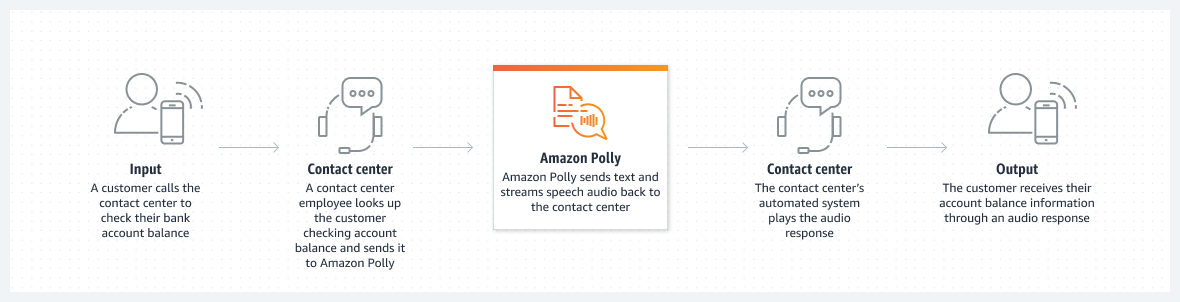
\includegraphics[scale=0.29]{polly-workflow.png}\\
	\end{center}
\end{frame}

\begin{frame}
	\frametitle{Where to use Amazon Polly}
	\begin{block}{}
		\begin{itemize}
			\vspace{1ex}
			\item Voice-Enabled Applications \vspace{1ex}
			\item Accessibility Tools \vspace{1ex}
			\item Media and Content Creation \vspace{1ex}
		\end{itemize}
	\end{block}		
\end{frame}

\begin{frame}
	\frametitle{Why use AWS Elastic Beanstalk}	
	\begin{block}{}
		\begin{itemize}
			\vspace{1ex}
			\item Natural Sounding Voices \vspace{1ex}
			\item Multiple Languages and Voices \vspace{1ex}
			\item Real-Time Speech \vspace{1ex}
		\end{itemize}
	\end{block}
	
\end{frame}


\begin{frame}
	\frametitle{Two-column slide}	
\end{frame}


\section{Second Section}

\begin{frame}
	\frametitle{Two-column slide}
	
\end{frame}




\end{document}